
\chapter{Blockchain Technology}
\label{chap:BCT}

Although the general pattern of linked data,
primarily using the terms '\textit{(One-Way) Hash Chain}' or '\textit{Merkle (Hash) Tree}' (\citet{Hu.2005}),
was known before the therm \gls{BCT}, the rise of Bitcoin,
enabled by \citeauthor{Nakamoto.2009}'s core paper in 2009 presenting the fundamental \gls{PoW} protocol, pushed \gls{BCT} into public attention.
In this thesis, \gls{BC} is from now on considered to be a (special) instance of the abstract term \gls{BCT} \label{sec:BCI}.
Additionally, \gls{BCT} is classified as a database technology.
More specific, \gls{BCT} "[...] is a form of distributed ledger technology, deployed on a peer-to-peer network where all data are replicated, shared, and synchronously spread across multiple peers" \cite[13]{Butijn.2020}.
Nowadays many different Blockchain network approaches exist, serving different (special) needs.
Before further details of the different \gls{BCT} approaches are presented, a short recapitulation is given, why all this effort is important. \\
Especially for cryptocurrencies, but also within all the other use cases (e.g.: \cite{Serada.2020}),
fraud in distributed trust-less environments shall be prevented \cite[1]{Xu.2019}.
Within cryptocurrencies, which are build upon \gls{BCT}, fraud is primarily known as \textbf{double spending} of money \cite[1]{Nakamoto.2009}.
This is why \citet{Nakamoto.2009}'s core paper was a breakthrough, as it offers "[...] a solution to the double-spending problem using a peer-to-peer network" \cite[1]{Nakamoto.2009}.
Generally, the "[...] blockchain protocol was designed to maintain a permanent traceable record between two parties that is transparent and
open to public scrutiny without the need of a middleman to authenticate transactions" \cite[483]{Gainsbury.2017}.
Hence \gls{BCT} is not only capable of dealing with money - it can also administer any kind of digital assets. \\
Consequently, in the context of online games, fraud 
can be equated with cheating - the illegal transactions which raise the probabilities to win a game.
Later on the space between providing needed information to keep the network alive and the need for hiding information,
not yet allowed to be revealed, will become small (see section \hyperref[sec:HiddenTransactionsPlusRandomization]{Hidden transactions \& Randomization}).
Especially under theses given circumstances, the prevention of double spending has to be ensured.
To understand the mechanics and techniques to prevent fraud better, this chapter offers core characteristics and an overview on recent mechanisms.
Six of them are briefly described:

\begin{enumerate}
	\item \textbf{Chain Structure} \\
	Data is stored in a linked chain, consisting of 'blocks of data'.
	The blocks are linked by fingerprints (hashes) of previous blocks and the write/update-process is cryptographically secured
	as shown in figure \ref{fig:BlockchainStructure} (alike \citet[654]{Lin.2017}).
	"The exception to this rule is the \textbf{Genesis Block}, which is the first block in the chain and has a predetermined hash"
	\cite[181]{Oliveira.2019}.
	The \textit{genesis block} will be of further importance in section \hyperref[sec:DataAllocationImprovements]{Data allocation improvements}
	of chapter \hyperref[chap:PoT]{Proof-of-Turn},
	\begin{figure}
		\centering{
			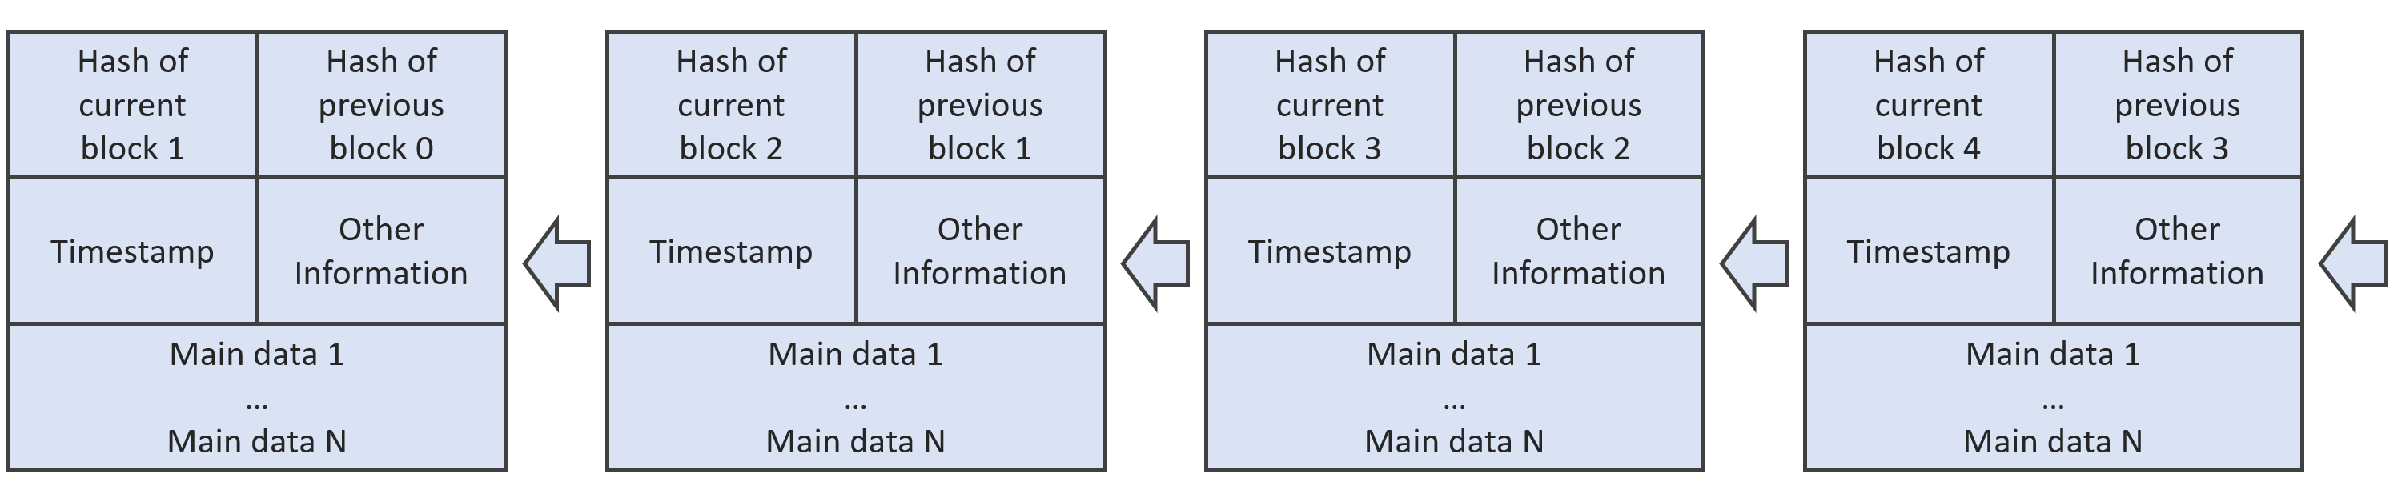
\includegraphics[width=.95\linewidth,keepaspectratio=true]{contents/images/BC_Stucture}
			\caption{Blockchain Structure (Adapted from \citet{Lin.2017})}
			\label{fig:BlockchainStructure}
		}
	\end{figure}

	\item \textbf{Decentralization, Distribution \& Disintermediation} \\
	"The blockchain is designed for distributing and synchronizing the data across multiple networks"
	\cite[6]{Sharma.2020}.
	"In traditional centralized transaction systems each transaction needs to be validated by a (trusted) third party (e.g., a bank). The decentralized workings of \gls{BCT} enables the direct transfers of digital assets between two counter parties without this third party leading to direct disintermediation" \cite[17]{Butijn.2020}.
	Although \gls{BC}s may be computed by only one peer, the benefit of \gls{BCT} stems from the network and the distribution of data itself,
	reducing the single point of failure \cite[79764]{Bodkhe.2020}.
	Finally all nodes strive to have the whole \gls{BC} stored to prevent fraud and to keep persistence with the other nodes \cite[79766]{Bodkhe.2020}.
	
	\item \textbf{Persistence \& Immutability} \\
	A \gls{BC} "[...] is a permanent record of transactions. Once a block is added, it cannot be altered. This creates trust in the transaction record" \cite[53]{SultanK..2018}.
	Generally data can only be invalidated by reference.
	Nevertheless, data can not be be deleted entirely \cite[88]{Sharma.2020}.
	Hence published data is immutable and distributed transparently throughout the network \cite[60-61]{Butijn.2020}.
	
	\item \textbf{Transparency} \\
	Moreover, until the last node is shut down, the \gls{BC}'s data is immutable published and all peers have the full data set \cite[88]{Sharma.2020}.
	As long as data in blocks is not encrypted to some peers, the BC is transparent and all peers possess the same collective knowledge \cite[483]{Gainsbury.2017}
	Additionally, as (new) data is always signed by a peer, information is traceable and transactions can be verified by all peers \cite[88]{Sharma.2020}.
	
	\item \textbf{Consensus Driven} \\
	Although there are special types, generally all nodes have the right to write blocks, if they follow the given ruleset \cite[54]{Dib.2018}.
	The given ruleset for adding data is called the \gls{CM} and differs regarding the \gls{BC}'s use case \cite[88]{Sharma.2020}.
	
	\item \textbf{Mining} \\
	The action of adding a new block to a \gls{BC} "is called mining
	and the nodes executing the calculations are referred to as miners in the Bitcoin nomenclature" \cite[4]{Butijn.2020}.
	The name stems from the reward - any type of tokens - granted by many \gls{CM}s.
	
\end{enumerate}
\noindent Before the usage of \hyperref[sec:BlockchainInGames]{Blockchain in Games} is introduced in the next chapter,
this chapter presents different \textit{network types and characteristics of \gls{BC}s} as well as commonly used \gls{CM}s.



\FloatBarrier

\section{Network types \& characteristics of Blockchains}
\label{sec:TypesOfBC}

In this section, \textit{accessibility of \gls{BC} networks} will be described before the \textit{layer structure} for pushing data is explained. 
Last, characteristics of \textit{Blocks, Transactions and Smart Contracts} are given.

\begin{enumerate}
	\item \textbf{Accessibility of BC networks} \\
	The following definitions deal with the accessibility of \gls{BC}s.
	Note that the following characteristics regarding accessibility do not influence
	the allocated storage space on the network's nodes - every node stores the full \gls{BC}.
	Generally it is distinguished between an \textbf{access policy} in the \textit{private/hybrid/public}-scheme
	and a \textbf{validation policy} in in the \textit{permissionless/permissioned}-scheme \cite[2]{Daniel.2019}.	
	The networks can be categorized as follows (Table \ref{tbl:BlockchainNetworkTypes}):
	
	\begin{enumerate}
		\item "In \textbf{public permissionless networks}, consensus mechanisms are required to be very strict due to the lack of trust between the participants.
		This is justified by the main feature of a public network, the equality between nodes.
		Once a network participant, the user receives a pair of cryptographic keys to sign and perform transactions.
		Any node can be a miner and participate in the consensus mechanism.
		The problems associated with public blockchains are the fees that must be paid to encourage users to participate in the network and to mine blocks;
		the concern with the network scalability; and the time interval to confirm the transactions.
		Such problems are related to the fact that public permissionless networks are collaborative environments and,
		therefore, depend on the benign behavior of nodes. Besides, for sensitive data networks,
		the fact that all information is available to everyone represents a challenge to data privacy.
		Due to the characteristics of public permissionless networks, costly consensus mechanisms are required" \cite[182]{Oliveira.2019}.
		\label{def:PublicPermissionlessBCNetworks}
		In this manner, \gls{BC} "[...] systems like Bitcoin and Ethereum are called permissionless, i.e. any node on the Internet can join and become a miner" \cite[1]{Angelis.2018}.
		
		\item To cure the needed computation power of \gls{BC} systems in \textit{public permissionless networks},
		"[...] \textbf{public permissioned networks} were developed to implement less costly consensus mechanisms on public networks.
		The difference between the public permissionless networks and the permissioned ones is the different roles that can be played by nodes in the network.
		In public permissioned networks, the node only participates of the network after proper verification of its identity" \cite[182]{Oliveira.2019}.
		\label{def:PublicPermissionedBCNetworks}
		
		\item "The \textbf{private permissionless networks} differ from public networks because they restrict the entry of participants.
		The private network is usually governed by a single institution or a set of institutions, which determine who are the nodes allowed to participate in the network.
		Participant nodes have equal functions and carry the same importance.
		Once authorized to participate in the network, the node can generate transactions and blocks, and participate in consensus" \cite[182]{Oliveira.2019}.
		\label{def:PrivatePermissionlessBCNetworks}
		
		\item "The \textbf{private permissioned networks} only allow some nodes to participate in the consensus process,
		and only a subset of these nodes can generate the next block" \cite[182]{Oliveira.2019}.
		\label{def:PrivatePermissionedBCNetworks}
	\end{enumerate}
	\begin{table}
		\centering
		\begin{tabularx}{0.48\textwidth}{ l | c | c }
			& Permissionless & Permissioned \\ \hline
			Public & \hyperref[def:PublicPermissionlessBCNetworks]{a)} & \hyperref[def:PublicPermissionedBCNetworks]{b)} \\ \hline
			Private & \hyperref[def:PrivatePermissionlessBCNetworks]{c)} & \hyperref[def:PrivatePermissionedBCNetworks]{d)} \\ \hline
			Hybrid & \hyperref[def:HybridPermissionlessBCNetworks]{e)} & \hyperref[def:HybridPermissionedBCNetworks]{f)} \\
			\hline
		\end{tabularx}
		\caption{Blockchain Network Types}
		\label{tbl:BlockchainNetworkTypes}
	\end{table}
	\noindent If \citet{SultanK..2018}'s definitions are considered as well,
	accessibility behaves within a grey scale between \textit{public}, \textit{private} and \textit{hybrid}. \\	
	\textbf{Public} \gls{BC}s ".. have no single owner; are visible by anyone;
	their consensus process is open to all to participate in;
	and they are full decentralized. Bitcoin is an example of a public blockchain" \cite[53]{SultanK..2018}. \\
	\textbf{Private} \gls{BC}s ".. use privileges to control who can read from and write to the blockchain.
	Consensus algorithms and mining usually aren’t required as a single entity
	has ownership and controls block creation" \cite[53]{SultanK..2018}. \\
	\textbf{Hybrid} \gls{BC}s ".. also known as consortium, these blockchains are public only to a privileged group.
	The consensus process is controlled by known, privileged servers using a set of rules agreed to by all parties.
	Copies of the blockchain are only distributed among entitled participants; the network is therefore only partly decentralized" \cite[53]{SultanK..2018}.
	\noindent Concluding, hybrid \gls{BC}s are operating in a public network, controlled by all nodes and hence do not fit into the bipolar private, public scheme.
	Hybrid entries are added as well:	
	\begin{enumerate}[start=5]
		\item \textbf{Hybrid permissionless} \gls{BC}s operate in a public network, but only an associated node can grant access \cite[53]{SultanK..2018}.
		No additional consensus has to take place \cite[53]{SultanK..2018}.
		This does not differ much from a \textit{public permissionless} \gls{BC}
		except the first entry barrier. \label{def:HybridPermissionlessBCNetworks}
		
		\item \textbf{Hybrid permissioned} \gls{BC}s, consequently, operate in a public network as well,
		but access needs to be granted by a majority of nodes (regarding a consensus protocol) \cite[53]{SultanK..2018}.	\label{def:HybridPermissionedBCNetworks}
	\end{enumerate}
	Within both hybrid types, again, the nodes are distributed and not controlled by any higher entity. \\
	
	From here on it is important to keep in mind that a round-robin consensus model is aimed for.
	The round-robin "[...] consensus model is usually used in \textit{permissioned} Blockchain. It allows nodes to take turn one by one for generating blocks" \cite[3]{Khan.2020}.
	Although the following \gls{PoT} mechanism (Section: \hyperref[chap:PoT]{Proof-Of-Turn}) could also be used for \textit{public permissionless} \gls{BC} networks,
	subsequent the focus will be on private as well as hybrid permissioned \gls{BC}s.
	
	\item \textbf{Layer structure} \\
	\gls{BCT} generally consists of four layers \cite[181]{Oliveira.2019},
	which pass data from the publishing (pushing) source node towards the global distribution throughout the network (Figure \ref{fig:LayersOfBlockchains}).
	\begin{figure}[!b]
		\centering{
			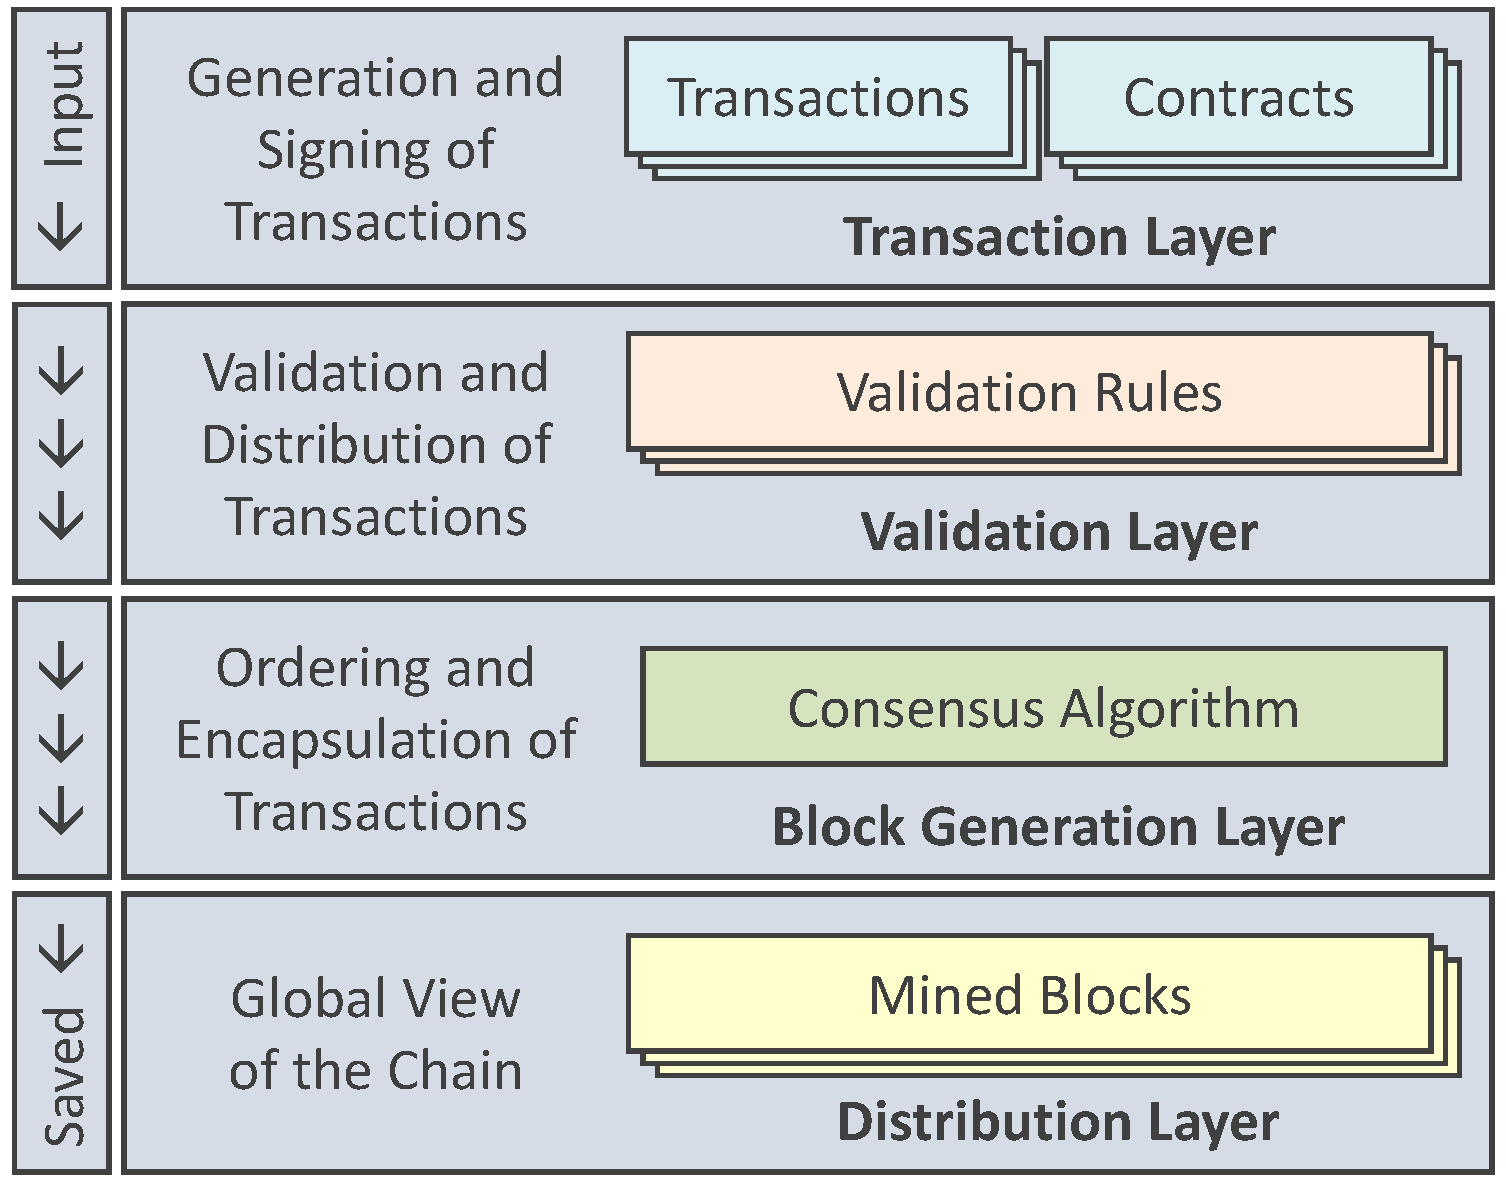
\includegraphics[width=.55\linewidth,keepaspectratio=true]{contents/images/BlockchainLayers}
				\caption{\citeauthor{Oliveira.2019}'s layers of \gls{BC} consensus}
			\label{fig:LayersOfBlockchains}
		}
	\end{figure}
	First, in the \textit{Transaction Layer}, new, local data from \hyperref[def_TransactionsAndSC]{transactions} is signed and given to the validation layer \cite[181]{Oliveira.2019}.
	Second, in the \textit{Validation Layer},
	each of the transactions are validated to the respective predefined rules \cite[181]{Oliveira.2019} - for example, defined by a \gls{SC}.
	As many/all nodes need to comply with the given data, the \hyperref[def_TransactionsAndSC]{transactions} are here (already) distributed among the nodes \cite[181]{Oliveira.2019}.
	\label{sec:SmartContract}
	Third, in the \textit{Block Generation Layer}, many \hyperref[def_TransactionsAndSC]{transactions} are combined and summed up in one block \cite[181]{Oliveira.2019}.
	This block is then passed into any \gls{CM} \cite[181]{Oliveira.2019}.
	This mechanism will distinguish the next added block and has to prevent hostile behavior of nodes (e.g. publishing a block against the consensus rules) \cite[54]{Dib.2018}.
	It can be seen as the gatekeeper for the data to be distributed.
	Please note that the wrapping of transactions into one block is primarily used to reduce computational effort \cite[1204]{Kim.2018},
	as some \gls{CM}s, like  Bitcoin's \gls{PoW}, are computation hungry \cite[11008]{Liu.2018}.
	Still, every transaction may also be appended individually to the \gls{BC}, which is only recommended along computationally lightweight \gls{CM}s.
	Different emendations regarding this manner are given in the following subsection \hyperref[sec:PerformanceImprovements]{Performance improvements}.
	Last, in the \textit{Distribution Layer}, all added blocks are 'finally' stored and the \gls{CM} 'ensures' that data,
	once written here, cannot be deleted \cite[182]{Oliveira.2019}. \\
	Finally, the "[...] data structure of a blockchain, whether public or consortium,
	corresponds to a linked list of blocks containing transactions also referred to as the 'ledger'" \cite[52]{Dib.2018}.

	\item \textbf{Blocks, Transactions and Smart Contracts} \\
	Next to the metadata the linked blocks, building the backbone structure of \gls{BCT}, consist of data, as shown in figure \ref{fig:BlockchainStructure}.
	More specifically all blocks can be seen as new, updated states of a \gls{BC} database \cite[1]{Danzi.52018}.
	Hence they are transactions, sometimes without direct impact or constraints to other nodes, sometimes even with mandatory consultation \cite[1]{Danzi.52018}.
	Moreover, a transaction can be "[...] an exchange of assets that is managed under the entity service’s rules" \cite[51]{SultanK..2018}.
	"These rules also form the basis for smart contracts.
	A smart contract is a set of logic rules in the form of a coded script which can be embedded into the blockchain to govern a transaction" \cite[51]{SultanK..2018}.
	The specific rules of \gls{SC}s and their validation are, understandably, implementation dependent and out of scope.
	Nevertheless, some game related meta-types of \gls{SC}s will be covered
	in the subsection \hyperref[sec:GSSCs]{Game specific smart contracts}
	of the upcoming	chapter \hyperref[chap:BlockchainInGames]{Blockchain in Games}.
\end{enumerate}
For now the skeleton of \gls{BCT} is known.
Thus, \gls{CM}s are now presented in further detail.



\FloatBarrier

\section{Consensus Mechanisms}
\label{sec:ConsensusMechanisms}

A major driver of progress in \gls{BCT} research lies within new \gls{CM}s, which unlock new fields of application.
As stated before, the \gls{CM}s are the gatekeepers for new data within each \gls{BC}.
A \gls{CM} can be grounded on some sort of \textbf{proof}, which has to be delivered by the pushing node \cite[106]{NguyenG.T..2018}.
Further, a \gls{CM} can be grounded on \textbf{votes} as well \cite[106]{NguyenG.T..2018}.
Generally, nodes who participate in the \gls{CM} need any incentive to meet the effort \cite[2]{Catalini.2016}.
Before some popular \gls{CM}s and their benefit system are described and discussed, two characteristics, \gls{BFT} and \gls{CF} need to be addressed: \label{sec:ByzantineFaultTolerance} \\
\textbf{\gls{BFT}} describes the share of nodes within a system, which are allowed to become hostile/unavailable
\textit{before the system is vulnerable} to break down, freeze or becomes prone for fraud \cite[1]{Gramoli.2017}. \label{sec:FinalStateSecurity} \\
\textbf{\gls{CF}} is a phrase to describe the \textit{indelible finality} of written data \cite[3]{Angelis.2018}.
Depending on the chosen \gls{CM}, data in the distribution layer (Figure \ref{fig:LayersOfBlockchains}, Layer 4) are 'only supposed to be final' \cite[3]{Angelis.2018}.
The low probability of \textit{non-finality-data} (e.g. in \gls{PoW}) makes data only implicitly 'consensus final' \cite[3]{Angelis.2018}.
Nevertheless, other \gls{CM}s - e.g. based on voting - provide data with (directly) secured final states \cite[3]{Angelis.2018}.
From a more formal perspective, \citet{Angelis.2018} uses \citet{Vukolic.2016}'s comparison on \gls{PoW} with \gls{BFT}-like approaches
"[...] introducing the distinguishing property of \textbf{consensus finality}: the impossibility of reaching consensus without fully distributed agreement.
In blockchain’s jargon, it amounts to the impossibility of having forks.
As expected, \gls{PoW} does not enjoy \textit{consensus finality} (as forks can happen), while all \gls{BFT}-like approaches does (all parties reach agreement before consensus)" \cite[3]{Angelis.2018}. \\
With this knowledge, \gls{CM}s by \textbf{proof} and \gls{CM}s by \textbf{votes} are given.
The reader has to be reminded that the list is limited on purpose due to manifold \gls{CM}s.

\subsection{Proof-of-Mechanisms}
There are several Proof-of-Mechanisms which differ in their characteristics. \label{sec:PbC}
To get an overview important/general mechanisms are introduced:

\begin{enumerate}
	\item \textbf{Proof-of-Work} \label{sec:PoW} \\
	The mechanism, which is supposed to be the most popular one, is the \gls{PoW} mechanism.
	It is used in the Bitcoin network and was introduced by Satoshi \citet{Nakamoto.2009}.
	Here, nodes have to solve mathematical problems to generate new blocks \cite[4]{Butijn.2020}.
	Pieces of the underlying \hyperref[sec:def_Cryptocurrency]{cryptocurrency} are used as
	incentives for finding the next suitable block (\citet[8]{Nakamoto.2009}; \citet[2]{Catalini.2016}).
	Hence the predominant motivation for the mining nodes to keep the network alive is supposed to be extrinsic.
	Additionally, the Bitcoin implementation adapts its energy consumption along the rising computation power
	within the network to generate a steady output of one block every ten minutes \cite[2254]{Ma.2020}.
	Generally an "[...] attacker would need the majority of the network’s computational power to rewrite history and calculate new blocks" \cite[3-4]{Demi.2021}. \\
	Still, "[...] each node needs to keep the history of all the transactions made in the network, so the storage space keeps increasing,
	and the number of transactions that can be processed by the network is quite limited, around 7 transactions per second [...]" \cite[81]{Besancon.2019}.
	Nevertheless Bitcoin scales along its stakeholders, who are not mining, pretty well - there is no limit in participants \cite[8]{Nakamoto.2009}.
	However, \gls{PoW} fails to reduce power consumption along an increasing mining network \cite[1-2]{Saleh.2020}.
	
	\item \textbf{Proof-of-Stake} \label{sec:DefPoS} \\
	\gls{PoS} was introduced to overcome the energy waste issue of \gls{PoW} (\citet[56]{Chaudhry.2018}; \citet{Narayanan.2018}).
	Whilst everyone is allowed to mine in the \gls{PoW} approach, the \gls{PoS} protects the network's
	stakeholders - those nodes with intrinsic motivation to keep the chain's integrity - from external nodes \cite[56]{Chaudhry.2018}.
	The \gls{PoS} \gls{CM}"[...] saves more energy as compared to the \gls{PoW} model.
	It is an energy efficient variant of \gls{PoW}.
	In \gls{PoS}, miners have to showcase and declare the ownership on a certain amount of currency.
	It is presumed that people with more cryptocurrency or coins would not attack the blockchain network" \cite[3]{Khan.2020}.
	Nevertheless, as nodes always seek to gain rewards, \gls{PoS} is running the risk of a \textit{Nothing-at-Stake problem},
	wherein "a validator will always update the ledger whenever given the opportunity even if the update necessarily perpetuates disagreement" \cite[2]{Saleh.2020}.
	The reduced power consumption stems from the reduced computation power (less mining nodes) within the network \cite[56]{Chaudhry.2018}.
	
	\item \textbf{Proof-of-Authority} \label{sec:DefPoA} \\
	Third, the \gls{PoA} approach, also known as \textit{Proof-of-Identity}, is presented:
	If a node wants to publish transactions, the node has to prove its "[...] identity and should be verifiable in the blockchain network.
	Basically, the publishing nodes are putting their \textbf{identity and reputation} for being a publishing node.
	Publishing node's reputation is directly linked to the publishing node's behavior.
	Any malicious activity by publishing [...] can \textbf{damage the reputation} of the node in the Blockchain network.
	Node reputation would increase if it acts in a manner that Blockchain users agreed with.
	Nodes with less reputation are \textbf{less likely to get the chance to publish a new block}. [...] 
	This model is preferred in permissioned blockchain for it requires a lot of trust on the nodes"	\cite[3]{Khan.2020}.
	
	\item \textbf{Proof-of-Elapsed-Time} \label{sec:DefPoET} \\
	For this mechanism special hardware (Software Guard Extensions - Intel SGX) is needed
	to create a Trusted Execution Environment called TEE, which works on the basis of exact timing \cite[55]{Dib.2018}.
	The \gls{PoET} Consensus Model "[...] selects random leader via election protocol. [...]
	A leader is selected to add the next block to the Blockchain in this model. [...]
	Every miner asks for the running code within the TEE for a waiting time and the miner with the lowest waittime becomes a leader node.
	TEE function can prevent tampering by any internal or external source.
	The only drawback in this consensus model is that it requires special hardware implementation" \cite[3-4]{Khan.2020}.
	
	\item \textbf{Proof-of-Play} \label{sec:DefPoP} \\
	Fifth, in the \gls{PoP} approach the interaction of a player behind a node is evaluated.
	"In the current \gls{PoP} design, the evaluation is adjusted according to the player’s ability.
	This provides a fair chance for everyone to pass through the evaluation stage with enough effort of their ability" \cite[23]{Yuen.2019}.
	Finally, the chosen node writes all parallel published data into one block \cite[23]{Yuen.2019}.
	
\end{enumerate}
\noindent Many of the presented Proof-of-Mechanisms were enhanced using several names, such as: \\
\textbf{Delegated Proof-of-Stake}, \textbf{Proof-of-Activity} (\gls{PoP}/\gls{PoS}-hybrid), \textbf{Proof-of-Achievement} (\citet{Komiya.2019}),
\textbf{Proof-of-Burn}, \textbf{Proof-of-Capacity} (or Proof-of-Storage), \textbf{Proof-of-Excellence} \cite[5]{King.2012}, \textbf{Proof-of-Existence}, \textbf{Proof-of-Importance},
\textbf{Proof-of-SequentialWork}, \textbf{Proof-of-Validation} (PoV), \textbf{Proof-of-Vote} as well as \textbf{Proof-of-WorkOrKnowledge} and \textbf{Proof-of-ZeroKnowledge}. \\
To dig deeper into most of these algorithms, \citet[5]{Butijn.2020} and \citet[3]{Angelis.2018} are recommended as starting points.
Nevertheless, these enhancements are considered to be out of scope due to their specificity. \\
Until now the permission to write a block was either dependent on available computation power (\gls{PoW}),
share of stake (\gls{PoS}), reputation within the network (\gls{PoA}),
exact timing (\gls{PoET}) or some kind of special effort (\gls{PoP}). \\
In Proof-of-Mechanisms much independence among the writing nodes is given - nodes are never asked to consent (explicitly) \cite[8]{Nakamoto.2009}.
Therefore competing versions of the \gls{BC}, known as \textbf{forks}, occur \cite[60]{Butijn.2020}.
"A user only needs to keep a copy of the block headers of the longest proof-of-work chain, which he can get by querying network nodes until he's convinced he has the longest chain, and obtain the Merkle branch linking the transaction to the block it's timestamped in" \cite[5]{Nakamoto.2009}.
A miner "[...] follows the \textbf{longest-chain rule} if she always chooses the last block of one of the longest chains" \cite[2]{Ewerhart.2020}.
This behavior, formally known as the \textit{Longest Chain Rule}, was first described by \citet{Courtois.2014}.
"Note that the \textit{longest-chain rule} is a class of strategies, rather than a single strategy" \cite[2]{Ewerhart.2020}.
The \textit{Longest Chain Rule} is the reason why blocks in some Proof-of-Mechanism \gls{BC}s may never reach $100$\% \gls{CF} \cite[3]{Angelis.2018}. \\
"Because of the possibility of forks, there is no such thing as absolute reliability of the data retrieved from the blockchain.
It is decreasingly high toward the most recent blocks data, as one only get the version of the ledger stored on a node at a given time,
so that a blockchain-specific time-dependent reliability weight has to be determined" \cite[62]{Dib.2018}.
Some Proof-of-Mechanisms have found their way around this flaw, such as \gls{PoET} and \gls{PoP}.
Nevertheless, on vote based (/consortium) \gls{BC}s, "[...] the use of adapted
consensus algorithm allows for “block finality”: once a block has been validated,
it remains on the main chain and forks are not allowed" \cite[54]{Dib.2018}.

\subsection{Vote-based Consensus}
\label{sec:VbC}
In contrast to \textit{Proof-of-Mechanisms}, \textbf{Vote-based-Mechanisms} - also
known as \textbf{consortium} mechanisms - only accept blocks which already reached consensus \cite[3]{Angelis.2018}. 
The accepted blocks reach a $100$\% \gls{CF} directly after approval \cite[3]{Angelis.2018}.
"The consensus is coordinated by the distributed nodes controlled by consortium partners which will come to a decentralized arbitration by voting. The key idea is to establish different security identity for network participants, so that the submission and verification of the blocks are decided by the agencies’ voting in the league without the depending on a third-party intermediary or uncontrollable public awareness. Compared with the fully decentralized consensus–Proof of Work (\gls{PoW}), vote-based consensus has controllable security, convergence reliability, only one block confirmation to achieve the transaction finality, and low-delay transaction verification time" \cite[466]{Kejiao.2017}. \\

Again there are multiple solutions:
\begin{enumerate}
	\item \textbf{Practical Byzantine Fault Tolerance Consensus Model} \label{sec:PracticalBFTCM} \\
	Malicious "[...] attacks, operator mistakes, and software errors are common causes of failure and
	they can cause faulty nodes to exhibit arbitrary behavior, that is, Byzantine faults" \cite[399]{Castro.2002}.
	The \gls{PBFT} is designed to prevent Byzantine faults.
	"It is mostly used in permissioned Blockchain such as in Hyperledger as it can manage up to 1/3 malicious byzantine replicas.
	In practical \gls{PBFT}, the next block is accepted in a round process.
	There are certain processes to follow in every round for choosing a primary node.
	The practical \gls{PBFT} model's process is classified into 3 well-defined phases: preprepared, prepared, and commit.
	For changing the state, the node should have at least 2/3 votes from all nodes.
	It will ensure that all nodes are recognizable and know with each and every node.
	[...] In \gls{PBFT} each node needs to inquire about other nodes"
	\cite[4]{Khan.2020}.
	\bigbreak
	
	\item \textbf{Ripple Consensus Model} \label{sec:RippleCM} \\
	This model will further be called \textbf{Ripple}.
	Every "[...] node needs to create a unique node list (UNL). All \gls{Ripple} nodes are part of UNL and are considered as reliable nodes for all other nodes to rely on them.
	No node are to go against UNL.
	\gls{Ripple} network encourages all nodes to communicate with various nodes available in that UNL to achieve consensus in the network.
	Every node in the UNL should make 40\% of overlap with all other nodes.
	In the \gls{Ripple} network, consensus could be achieved in a couple of rounds where all nodes understand the responsibility for assembling the transaction
	with the state of the candidate set in a "a well-known data structure" and transmit its candidate sets to nodes in the current UNL.
	Nodes are responsible for validating the transaction, vote for a specific transaction and transmit the votes to the network based on the results of the collective votes.
	Every node filters out its candidate set and transaction receiving the highest votes are transferred to coming round of consensus.
	Right after achieving the 80\% votes of candidates set from every node available in the UNL then that particular candidate set becomes the ledger in \gls{Ripple} term.
	Another round of consensus would start with the new and pending transaction which could not get accepted.
	Consensus in the whole network can only be achieved after every sub-network achieves consensus"
	\cite[4]{Khan.2020}.
	
	\item \textbf{Tendermind Consensus Model} \label{sec:TendermindCM} \\
	\citet[4]{Khan.2020} summarizes the \gls{TCM} from \cite{Kwon.2014} as follows:
	\gls{TCM} "[...] is another variant of \gls{PBFT} model which mostly works with permissionless Blockchain.
	In this model, clients have the privilege of directly creating a new transaction to the nodes.
	The clients in this model utilize the gossip protocol to broadcast the transaction for the validating nodes.
	Within the Brach broadcast pattern, the progression would be done with the external validating situation so
	validating nodes are required to collect the transaction by gossip right before it gives a right to include the transaction in the block. \\
	The significant difference between Tendermind and \gls{PBFT} is that it continuously rotates the leader node right.
	Tendermind takes \gls{PBFT} view change mechanism into the common case pattern.
	Here this shows as it is waiting to timeout, and validating nodes wait for the leader node to convey the first message in the Bracha broadcast pattern.
	which is more relevant to the view change the timer in \gls{PBFT}.
	As the timer expires validating nodes vote to a nil block and validating nodes take part n the Bracha Broadcast message pattern on a continuous basis.
	The Tendermind was suffering from many issues and the obvious one was livelock, presenting locking and unlocking votes by validating nodes."
	
\end{enumerate}

\noindent The last two approaches which are covered are enhancements of above given \gls{CM}s: \textit{MultiChain} and \textit{Child-chains}. \\
\textbf{MultiChain} "[...] enforces a round robin schedule, in which the permitted miners must create blocks in rotation
in order to generate a valid blockchain" \cite[7]{Greenspan.2015}. \label{def:MultiChain}
Hereby the round robin is implicitly enforced regarding a value called \textit{mining diversity} \cite[7]{Greenspan.2015}.
"A value of 1 ensures that every permitted miner is included in the rotation, whereas 0
represents no restriction at all. In general, higher values are safer, but a value too close to 1 can
cause the blockchain to freeze up [...]"
\cite[7]{Greenspan.2015} due to inactive miners - the network stalls.
If a network split occurs, "[...] the fork with the longer chain will be adopted as the global consensus.
The diversity threshold ensures that the longer blockchain will belong to the island
containing the majority of permitted miners, since the other island’s chain will quickly freeze up"
\cite[8]{Greenspan.2015}.
\textit{MultiChain} is only an example for a general round robin approach. \\
\textbf{Child-chains} can be used with every \gls{BCT} and presuppose parallel \gls{BC} threads.
Further, \textit{side-chains} assume that there are transactions which necessarily belong on the main
tread (primary chain) and others which do not need to be stored on the primary chain \cite[1206]{Kim.2018}.
Therefore the ladder can reduce the load on the \textit{primary chain}.
Here transactions which are written to the \textit{primary chain} are called \textit{on-chain} and those written to any \textit{sidechains}, \textit{off-chain}.
"In a traditional on-chain transaction, each transfer would have to be validated by all peers in the network before the transfer is labelled as complete, which keeps it very slow.
In contrast, in an off-chain transfer, not all peers need to wait for the transfer to be verified before it is labelled as successful or complete" 
\cite[15]{Sharma.2020}. \\
Concluding, \textit{MultiChain} seeks a reduction of needed overall computation power and \textit{child-chains} reduce the reconciliation effort.
Last, as \textit{child-chains} are not tied to a special \gls{CM}, they are covered in the following subsection \hyperref[sec:PerformanceImprovements]{Performance improvements}.
A comparison of the given \gls{CM}s follows thereafter.



\subsection{Performance Improvements}
\label{sec:PerformanceImprovements}
Next to the general functionalities to achieve consensus, there are some scalability solutions, which can be applied to multiple upper level \gls{CM}s.
On this topic, \citet[1204]{Kim.2018} offer five categories of improvement-methods they found in their survey.
Whilst On-chain, Off-chain and Child-chain improvements operate within a main-chain's network (only),
Side-chain and Inter-chain try to connect \gls{BC}s out of different networks.
The key facts are given briefly:

\begin{enumerate}
	\item "The \textbf{on-chain} solution refers to methods that increase scalability by modifying only elements within a blockchain" \cite[1204]{Kim.2018}.
	One prominent example would be to increase the number of transactions within one block until it is considered a 'Big block' \cite[1204]{Kim.2018}. \\
	In the following specific case, the "[...] Bitcoin Core protocol limits blocks to 1 MB in size.
	Each block contains at most some 4,000 transactions.
	Blocks are added to the blockchain	on average every 10 minutes,
	therefore the transaction rate is limited to some 7 transactions per second" \cite[1]{Goebel.2017}.
	\begin{table}[!b]
		\centering
		\begin{tabularx}{0.80\textwidth}{ l | c | c | c }
			& Transaction / second & Transactions / block & Block size \\ \hline
			Bitcoin Core & $7$ & $4.000$ & $1$ MB \\ \hline
			Big block (1) & $70$ & $40.000$ & $10$ MB \\ \hline
			Big block (2) & $700$ & $400.000$ & $100$ MB \\ \hline
		\end{tabularx}
		\caption{Blockchain Blocksize}
		\label{tbl:BlockSize}
	\end{table}
	If a block was allowed to be bigger than the traditional 1 MB of Bitcoin Core, it would enable more
	transactions to be processed in the same amount of time (Table \ref{tbl:BlockSize}: 'Big block' 1 \& 2),
	as solving the \gls{PoW}'s mathematical mining problem is barely constraint to the actual block size (\cite{Zhang.2018}).
		
	\item "The \textbf{off-chain} solution is to improve the scalability by processing the transactions at outside the blockchain.
	This is also called a \textbf{state-channel} solution, because it maintains the state of the main-chain and applies the last state that has been processed in the other channel" \cite[1205]{Kim.2018}.
	In other words, in "[...] a traditional \textit{on-chain} transaction, each transfer would have to be validated by all peers
	in the network before the transfer is labelled as complete, which keeps it very slow.
	In contrast, in an \textit{off-chain} transfer, not all peers need to wait for the transfer to be verified before it is labelled as successful or complete" \cite[15]{Sharma.2020}.
	'The Bitcoin Lightning Network' (\citet{Poon.2016}), Sprites (\citet{Miller.2017}) and game channels (\citet{Kraft.2016}) fit into this category.
	All three papers split transactions from the main chain, starting with an introducing interaction just to merge the results of the sidechain branch back into the main chain later on.
	In figure \ref{fig:ChainImprovements} temporary off-chains can be seen. 
	Whilst the main-chain is managed by all nodes of the network,
	the \textit{off-chain state channels} are only governed by the (two) affected nodes.
	Generally, \citet{Poon.2016} can be seen as the founders of
	this idea and \citet{Miller.2017}'s research aims to further improve the speed.
	As those two are located in the cryptocurrency business only, they are out of scope.
	Regarding \gls{BCT} in games, \citet{Laneve.2019} (p. 27) state that this "[...] approach gives the developers all the flexibility they need with proven infrastructures while decentralising only the parts that need it".
	Although \citet{Kraft.2016} is using \gls{BCT} based on a cryptocurrency in both on-chain as well as off-chain transactions, he is located within online gaming business.
	Therefore \citet{Kraft.2016}'s research will become important later on.
	
	\begin{figure}[!b]
		\centering{
			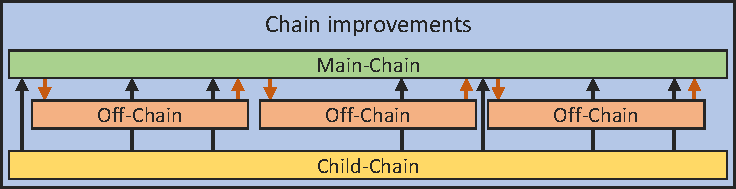
\includegraphics[width=.95\linewidth,keepaspectratio=true]{contents/images/ChainImprovements}
			\caption{Off-Chain \& Childchain}
			\label{fig:ChainImprovements}
		}
	\end{figure}
	
	\item "The \textbf{child-chain} solution has a parent-child structure, processes the transactions in the child-chain, and records the results in the parent-chain" \cite[1206]{Kim.2018}.
	On the one hand, this can be used for further improvements on cryptocurrency transactions (\citet[1206]{Kim.2018}),
	on the other hand, special transactions can be stored on the child-chain,
	which are only transferred to the parent-chain on fulfilled
	smart contracts (see \hyperref[sec:DataAllocationImprovements]{Data allocation improvements} in chapter \hyperref[chap:BlockchainInGames]{Blockchain in Games}).
	Consequently, in figure \ref{fig:ChainImprovements} a sample permanent \textit{child-chain} 
	is 'every once in a while' used to push certain data into the \textit{main-chain} (dark arrows).
	
	\item "The \textbf{side-chain} approach is to exchange assets of different blockchains with each other.
	And their goal is to bring the function of another blockchain into the current blockchain" \cite[1205]{Kim.2018}.
	In the first place, two \gls{BC}s with different \gls{CM}s are combined to obtain the advantages of both approaches, such as using smart contracts of Ethereum together with Bitcoin's cryptocurrency (\citet{Kim.2018}, p. 1205-1206).
	Here, prominent example which is mentioned more often in the literature is \citet{Back.2014}'s paper about 'Pegged Sidechains'. \\
	In figure \ref{fig:ChainImprovements} the side-chain approach is used,
	if one of the layers needs a divergent \gls{CM} to serve special service characteristics.
	In section \hyperref[sec:Interoperability]{Interoperability} in chapter \hyperref[chap:PoT]{Proof-of-Turn}
	the \gls{PoT} \gls{CM} serves as as an off-chain/side-chain solution for a \gls{PoW} \gls{BC}
	(e.g. for an ecosystem's in-game currency), whilst the
	\gls{PoT} \gls{CM} is served by an off-chain/side-chain \gls{PBFT} \gls{BC} to enable straight forward and lightweight voting (Figure \ref{fig:MultiLayerBC}).
	
	\item "The \textbf{inter-chain} method is a way to enable communication among the various blockchain" \cite[1206]{Kim.2018}.
	Inter-chain is very similar to the side-chain approach and tries to make e.g. Litecoin and Bitcoin interoperable \cite[1206]{Kim.2018}.
	Hence, the inter-chain method can be seen as the infrastructure technology for implementing the side-chain \cite[1206]{Kim.2018}.
\end{enumerate}
Further advantages and disadvantages, here out of scope, can be taken from \citet{Kim.2018} (p. 1206, Table 1., A comparative analysis table of the scalability issues).
Concluding, if possible, a novel \gls{CM} shall offer the possibility to be interoperable, as \citet[81]{Besancon.2019} states that the need for interoperability
"[...] can be found at multiple levels: a) between different BC, b) between different projects running on the same BC, and c) between BC and other technologies used to create decentralized applications." \\
Later on, during the design of \gls{PoT}, \textbf{on-chain} improvements in regards of number of blocks written within a given time slot,
the \textbf{off-chain} method regarding interoperability,
\textbf{child-chains} to counterweight in-game mechanics as well as 
\textbf{side-chain} solutions for mixing \gls{CM} characteristics will be of interest.

\FloatBarrier



\subsection{Comparison of Consensus Mechanisms}

\begin{table}
	\centering
	\begin{tabularx}{0.575\textwidth}{ c | c | c }
		\textbf{Proof based} & \textbf{Write} & \textbf{\gls{BFT}} \\
		\textbf{\gls{CM}s} & \textbf{permission} & \\ \hline \hline
		\gls{PoW} & Heavy computation & \textless $25$ \% \\ \hline
		\gls{PoS} & Stakeholder & \textless $50$ \%  \\ \hline
		\gls{PoA} & Authority & \textless $51$ \%  \\ \hline
		\hyperref[sec:MultiChain]{MultiChain} & Round Robin & \textminus  \\ \hline
		\gls{PoET} & Time & \textminus \\ \hline \hline
	\end{tabularx}
	\caption{Proof based consensus mechanisms \cite[5]{Khan.2020}}
	\label{tbl:SumConsensusMechanisms_1}
\end{table}

\noindent To sum up the given \gls{CM} overview, Table \ref{tbl:SumConsensusMechanisms_1} (Proof based \gls{CM}s) and Table \ref{tbl:SumConsensusMechanisms_2} (Vote based \gls{CM}s)
show the mechanism's characteristics regarding \textit{write permissions} and \textit{\gls{BFT}}.
Values are taken from \citet[5]{Khan.2020}, which match
values from \citet[55]{Dib.2018}.

\begin{table}
	\centering
	\begin{tabularx}{0.55\textwidth}{ c | c | c }
		\textbf{Vote based} & \textbf{Write} & \textbf{\gls{BFT}} \\
		\textbf{\gls{CM}s} & \textbf{permission} & \\ \hline \hline
		\gls{PBFT} & Vote rounds  & \textless $33.3$ \% \\ \hline
		\gls{Ripple} & Leader rotation & \textless $20$ \%  \\ \hline
		\gls{TCM} & Leader rotation & \textless $33.3$ \%  \\ \hline
		\hline
	\end{tabularx}
	\caption{Vote based consensus mechanisms \cite[5]{Khan.2020}}
	\label{tbl:SumConsensusMechanisms_2}
\end{table}

\noindent Although values in Table \ref{tbl:SumConsensusMechanisms_3} (Additional \gls{CM}s) are only anticipated, they are given to complete the list.
\begin{table}
	\centering
	\begin{tabularx}{0.75\textwidth}{ c | c | c }
		\textbf{Proof based} & \textbf{Write} & \textbf{\gls{BFT}} \\
		\textbf{\gls{CM}s} & \textbf{permission} & \\ \hline \hline
		\gls{PoP} & Effort in game & \textminus  \\ \hline
		\gls{PoT} & Round Robin, turn (time)  & Implementation \\
		 & and special rules & dependent \\ \hline
	\end{tabularx}
	\caption{Additional consensus mechanisms}
	\label{tbl:SumConsensusMechanisms_3}
\end{table}
\noindent Table \ref{tbl:SumConsensusMechanisms_1}, \ref{tbl:SumConsensusMechanisms_2} and
\ref{tbl:SumConsensusMechanisms_3} show the different approaches, which can be used to model a game specific \gls{CM}.
All values, to the author's knowledge, are given for plain \gls{CM}s without enhancements from the previous section \hyperref[sec:PerformanceImprovements]{performance improvements}. \\
Nevertheless, the "[...] existing proof-of-based models seem to be supporting open participation
but they are not suitable for the real-time applications where immediate
transaction finality and high transaction rates are the main requirement" \cite[6]{Khan.2020}.
Finally, as all theses mechanisms are solving storage related issues, the '\textit{CAP theorem}' as described by \cite{Brewer.2012}, has to be mentioned as well.
In a distributed data store, such as \gls{BCT}, out of the three following properties \gls{C}, \gls{A} and \gls{P} only two can be ensured \cite[6]{Angelis.2018}.
Thus either \gls{C}$+$\gls{A}, \gls{C}$+$\gls{P} or \gls{A}$+$\gls{P} can fully be met \cite[6]{Angelis.2018}.
Additionally, "[...] an Internet-deployed permissioned blockchain has to tolerate these adverse situations:
(i) periods where the network behaves asynchronously;
(ii) a (bounded) number of Byzantine authorities aiming at hampering availability and consistency" \cite[7]{Angelis.2018}.
Consequently from (i), there is no way around \gls{P} and a trade off between \gls{C} and \gls{A} has to be found \cite[7]{Angelis.2018}.
The CAP theorem will further be covered in chapter \hyperref[chap:PoT]{Proof-of-Turn}, section \hyperref[sec:CAPtheorem]{CAP Theorem measurement}. \\

\noindent Additionally, from the given information it can be concluded that \textit{forks are expensive}.
Consequently, designing a \gls{CM} without forks or \textit{diminished computation in vain} along forks is strived for to increase energy efficiency and to reduce network traffic as well as inconsistencies.
Still, to meet the needs of speed/throughput the interoperability with \textbf{off-chain}, \textbf{side-chain} and \textbf{child-chain} improvements is beneficial. \\
Revising the research question, \textit{"What is the best fitting \gls{BCT} \gls{CM} to cover an asynchronous game play scenario?"}, the answer is not clear, yet.
If there was a novel \gls{CM} design, the lowest possible consultation in regards of the given scenario is aimed for.
This solution does not necessarily need an attached cryptocurrency. \\
In chapter \hyperref[sec:PoT]{Proof-of-Turn} the following characteristics will become important:
\begin{enumerate}
	\item \textit{Round Robin}, in regards of reducing the \textit{permissioned writing node} down to one
	using a fixed succession.
	\item \textit{Time}, not as strict as in \gls{PoET}, but not negligible.
	\item \textit{\gls{BFT}}, to an (at least) reasonable extend of \textless $33.3$ \%, or more (implementation dependent).
	\item \textit{\gls{CF}}, both in the fashion of short-termed forks as well as possible long-termed rewrites of the blockchain.
	\item \textit{\gls{PoP}}, in regards of the final scope of the \gls{PoT} \gls{CM} for games.
	\item \textit{Off-chain}, as stated in \citet{Kraft.2016}'s paper using the phrase \textit{Game Channel}.
	\item \textit{Child-chain(s)/Side-chain(s)}, in the manner of organizing different types of transactions.
	\item \textit{Interoperability}, as an additional desirable characteristic.
\end{enumerate}

\noindent Still, before getting into the details of the \gls{PoT} \gls{CM} in chapter \hyperref[chap:PoT]{Proof-of-Turn},
the next chapter \hyperref[sec:BlockchainInGames]{Blockchain in Games} will list characteristics \gls{BCT} needs to fulfill in general to serve turn based games.


